\documentclass[10pt]{article}
\usepackage[utf8]{inputenc}
\usepackage[T1]{fontenc}
\usepackage{hyperref}
\hypersetup{colorlinks=true, linkcolor=blue, filecolor=magenta, urlcolor=cyan,}
\urlstyle{same}
\usepackage{amsmath}
\usepackage{amsfonts}
\usepackage{amssymb}
\usepackage[version=4]{mhchem}
\usepackage{stmaryrd}
\usepackage{graphicx}
\usepackage[export]{adjustbox}
\graphicspath{ {./images/} }

\title{Recalculating Sargent and Wallace's "Some Unpleasant Monetarist Arithmetic"* }

\author{Iván Werning\\
MIT}
\date{}


%New command to display footnote whose markers will always be hidden
\let\svthefootnote\thefootnote
\newcommand\blfootnotetext[1]{%
  \let\thefootnote\relax\footnote{#1}%
  \addtocounter{footnote}{-1}%
  \let\thefootnote\svthefootnote%
}

%Overriding the \footnotetext command to hide the marker if its value is `0`
\let\svfootnotetext\footnotetext
\renewcommand\footnotetext[2][?]{%
  \if\relax#1\relax%
    \ifnum\value{footnote}=0\blfootnotetext{#2}\else\svfootnotetext{#2}\fi%
  \else%
    \if?#1\ifnum\value{footnote}=0\blfootnotetext{#2}\else\svfootnotetext{#2}\fi%
    \else\svfootnotetext[#1]{#2}\fi%
  \fi
}

\begin{document}
\maketitle
FEDERAL RESERVE BANK of MINNEAPOLIS

\section*{QUARTERLY REVIEW}
NOVEMBER 2024\\
Recalculating Sargent and Wallace's "Some Unpleasant Monetarist Arithmetic"

Iván Werning

\section*{Argentina at a Crossroads}
Tobias Martinez Gonzalez\\
Juan Pablo Nicolini

\section*{FEDERAL RESERVE BANK of MINNEAPOLIS}
\section*{Quarterly Review vol. 44, No. 3 \\
 ISSN 0271-5287}
\href{https://doi.org/10.21034/qr}{https://doi.org/10.21034/qr}. 4431

This publication primarily presents economic research aimed at improving policymaking by the Federal Reserve System and other governmental authorities.

The views expressed herein are those of the authors and not necessarily those of the Federal Reserve Bank of Minneapolis or the Federal Reserve System.

SENIOR VICE PRESIDENT AND DIRECTOR OF RESEARCH: Andrea Raffo\\
EDITOR: Juan Pablo Nicolini\\
ARTICLE Editor: James Holt\\
TECHNICAL SUPPORT: Amol Amol

The Quarterly Review is published by the Research Division of the Federal Reserve Bank of Minneapolis.\\
This has become an occasional publication; however, it continues to be known as the Quarterly Review for citation purposes. Subscriptions are available free of charge. To subscribe to the journal and be automatically notified whenever a new issue is published, please sign up at \href{https://www.minneapolisfed.org/economic-research/}{https://www.minneapolisfed.org/economic-research/}

Quarterly Review articles that are reprints or revisions of papers published elsewhere may not be reprinted without the written permission of the original publisher. All other Quarterly Review articles may be reprinted without charge. If you reprint an article, please fully credit the source-the Minneapolis Federal Reserve Bank as well as the Quarterly Review-and include with the reprint a version of the standard Federal Reserve disclaimer (italicized above). Also, please send one copy of any publication that includes a reprint to the Research Division of the Federal Reserve Bank of Minneapolis.



\begin{abstract}
This note revisits and extends the seminal analysis by Sargent and Wallace, originally framed in terms of money growth rates. Here, I reexamine their model through two complementary lenses, treating the policy instrument as either (i) a sequence of interest rates or (ii) a sequence of seigniorage. In the process, I revisit Sargent and Wallace's "spectacular" example and offer a variant that strengthens their conclusions.
\end{abstract}

Sargent and Wallace (1981) warned us against the perils of considering monetary and fiscal policies in isolation. Indeed, their paper taught us that monetary policy may be severely constrained by fiscal policy. Armed with a truly minimalist model, featuring a money demand and government budget constraint, they derived two insightful results for cases where the path for fiscal deficits does not adjust to monetary policy changes-that is, under fiscal dominance. First, they showed that efforts to lower current inflation via lower money growth may succeed in the short run but lead to higher inflation in the future. Second, in some cases these very efforts backfire spectacularly: delivering higher inflation in all periods!

This note celebrates their seminal paper. My main goal is to faithfully review the essence of the original, while providing another perspective that complements and compliments their analysis. Sargent and Wallace parameterized monetary policy using money growth rates. Instead, I study policy from two flexible perspectives, treating the policy instrument as either (i) the path of interest rates or (ii) the path of seigniorage. I also review the nature of Sargent and Wallace's "spectacular" example and offer a variant that reinforces its interpretation.

\footnotetext{*This work evolved from teaching notes used at MIT for over 10 years and was first shaped into a note during a 2021 conference titled "Monetary/Fiscal Interactions 40 Years after 'Unpleasant Monetarist Arithmetic'" organized by the Minneapolis Federal Reserve Bank. I thank Juan Pablo Nicolini, Marco Bassetto and Tom Sargent for helpful comments.
}The first approach, which uses interest rates, offers several advantages. First, it is the dominant way to discuss monetary policy these days. Second, in the present setup it is directly related to inflation, the outcome of interest. Third, following Friedman and the optimal taxation literature, interest rates, not inflation, most accurately represent a tax rate on real money holdings. From this vantage point, the first Sargent-Wallace result relates to the public finance principle that if a tax rate (interest rate, and, thus, inflation) is lowered, then other tax rates (interest rates and, thus, inflation rates) must typically be raised to maintain budget balance. Their second result is based on a "spectacular" example where inflation can be increased or decreased in all periods. Using my analysis, this situation can be seen from a public finance perspective as one on the "bad" side of a Laffer curve. As it turns out, the Laffer curve that formalizes this idea is not the traditional one, but a close cousin defined in terms of interest rates.

The second approach, working with seigniorage, is attractive at a conceptual level since it captures the essence of a fiscally dominant regime. In such a regime, the central bank must deliver a certain present value of real transfers to the Treasury. Monetary policy can choose the timing of seigniorage, but is subject to a present value. I provide a formula for inflation as a discounted sum of current and future seigniorage. By linking inflation directly to seigniorage, this formula expresses a fiscal dominance perspective of inflation. Comparing the discounting in my formula with the real interest rate in the government budget constraint brings forth the two core Sargent-Wallace results. When the discount rate in the formula is lower, inflation is strongly dependent on future seigniorage and, as a result, can be lowered in all periods by tilting seigniorage toward the present, as in Sargent-Wallace's first result. Otherwise, a tradeoff emerges between current and future inflation, as in Sargent-Wallace's first result.

The two perspectives and characterizations I offer are fully consistent with each other: the discount rate turns out to be lower than the interest rate on the bad side of the interest-rate Laffer curve.

\section*{Present Value Conditions}
The model boils down to four equations: a nominal government budget constraint, the definition of seigniorage from money issuance, a money demand function and the Fisher equation for interest rates,

\begin{equation*}
B_{t, t+1}+P_{t} s_{t}=P_{t} d_{t}+\left(1+i_{t-1, t}\right) B_{t-1, t}
\end{equation*}

\section*{FEDERAL RESERVE BANK OF MINNEAPOLIS}
QR

\begin{equation*}
\begin{gathered}
s_{t}=\frac{M_{t, t+1}-M_{t-1, t}}{P_{t}} \\
\frac{M_{t, t+1}}{P_{t}}=L_{t}\left(i_{t, t+1}\right) \\
1+i_{t, t+1}=\left(1+r_{t, t+1}\right)\left(1+\pi_{t, t+1}\right)
\end{gathered}
\end{equation*}

for $t=0,1, \ldots$ where $P_{t}$ is the price level, $d_{t}$ is an exogenous real fiscal deficit (purchases plus transfers minus taxes), $B_{t, t+1}$ and $M_{t, t+1}$ are nominal bonds and cash money held by households between periods $t$ and $t+1, \pi_{t, t+1}=P_{t+1} / P_{t}-1$ is inflation, $i_{t, t+1}$ is the nominal interest rate, and $r_{t, t+1}>0$ is the real rate between $t$ and $t+1$. We also impose a standard no-Ponzi condition that $q_{t} B_{t, t+1} / P_{t} \rightarrow 0 .{ }^{1}$ The demand for money is a non-increasing function $L_{t}(i)$ of the nominal interest rate. Adopting a monetarist perspective, the real interest rate sequence $\left\{r_{t, t+1}\right\}$ is assumed exogenous.

The variables $B_{-1,0}, M_{-1,0}$ and $i_{-1,0}$ are given predetermined variables. In addition, Sargent and Wallace assume $M_{0,1}$ is given. ${ }^{2}$ Define $\omega_{0} \equiv\left(1+i_{-1,0}\right) B_{-1,0} / M_{-1,0}$ and $1+\Delta_{0} \equiv M_{0,1} / M_{-1,0}{ }^{3}$

Two Equivalent Present Value Conditions. Iterating on the government budget constraint gives the present value budget constraint (Appendix provides a full derivation)

\begin{equation*}
\sum_{t=1}^{\infty} q_{t} s_{t}+\frac{\Delta_{0}-\omega_{0}}{1+\Delta_{0}} L_{0}\left(i_{0,1}\right)=D \tag{1}
\end{equation*}

where $q_{t} \equiv\left(1+r_{0,1}\right)^{-1}\left(1+r_{1,2}\right)^{-1} \cdots\left(1+r_{t-1, t}\right)^{-1}\left(\right.$ with $\left.q_{0}=1\right)$ and $D \equiv \sum_{t=0}^{\infty} q_{t} d_{t}$ are exogenously given. The first summation term represents the present value of seigniorage from $t=1$ onwards. The second term captures initial seigniorage $s_{0}=M_{-1,0} \Delta_{0} / P_{0}$ minus the real value of government debt $M_{-1,0} \omega_{0} / P_{0}$. In equilibrium, the initial price level is $P_{0}=M_{-1,0}\left(1+\Delta_{0}\right) / L_{0}\left(i_{0,1}\right)$. Putting these expressions together gives $\left(\Delta_{0}-\omega_{0}\right) /(1+$ $\left.\Delta_{0}\right) L_{0}\left(i_{0,1}\right)$.

An equivalent expression for the intertemporal budget constraint is (Appendix provides a full derivation)

\begin{equation*}
\sum_{t=0}^{\infty} q_{t} \frac{i_{t, t+1}}{1+i_{t, t+1}} L_{t}\left(i_{t, t+1}\right)-\frac{1+\omega_{0}}{1+\Delta_{0}} L_{0}\left(i_{0,1}\right)=D \tag{2}
\end{equation*}

The first summation term now represents the present-value of the financial benefit of using money $M_{t, t+1}$ instead of interest-bearing debt $B_{t, t+1}$. From the government's perspective,\\
both represent liabilities but with different rates of return: 0 for money and $i_{t, t+1}$ for bonds. The difference in returns given by the nominal rate $i_{t, t+1}$ then acts a tax on money relative to bonds, as Milton Friedman famously explained. ${ }^{4}$ In (2) the second term captures the initial real value of all government liabilities from money and debt, given by $M_{-1,0}(1+$ $\left.\omega_{0}\right) / P_{0}$ and the initial price level $P_{0}$ dilutes the real value and is given as before by $P_{0}=$ $\left(1+\Delta_{0}\right) M_{-1,0} / L\left(i_{0,1}\right)$. Putting these two expressions together explains the term $(1+$ $\left.\omega_{0}\right) L_{0}\left(i_{0,1}\right) /\left(1+\Delta_{0}\right) .{ }^{5}$

Bassetto and Sargent (August 2020) also discuss a version of (2)—but without substituting out for the equilibrium $P_{0}$-and use it to discuss various ways in which fiscal and monetary policy are intertwined.

Two Laffer Curves. The Laffer curve is traditionally defined in terms of seigniorage for a stationary scenario with constant money demand and constant inflation by

\begin{equation*}
\frac{\bar{\pi}}{1+\bar{\pi}} L(\bar{\pi}),
\end{equation*}

where I have abused notation to write $L$ as a function of $\pi$, with $1+i=(1+\pi)(1+r)$ and $r$ taken as given. These traditional Laffer curves capture the real flow value of new money issuances.

Breaking with this tradition, constraint (2) suggests treating

\begin{equation*}
\frac{i_{t, t+1}}{1+i_{t, t+1}} L_{t}\left(i_{t, t+1}\right)
\end{equation*}

as an alternative interest-rate Laffer curve. This alternative Laffer curve has the advantage of not requiring stationarity nor a constant inflation rate.

Figure 1 illustrates both Laffer curves for a linear demand curve based on the Sargent and Wallace example. Since $r>0$, the interest-rate Laffer curve lies on top of the traditional one. Laffer curves may or may not have a peak ${ }^{6}$, but if a peak exists for the traditional Laffer curve, then the peak for the alternative Laffer curve occurs at a lower inflation rate, as illustrated in the figure. Thus, being on the bad side of this Laffer curve is more likely.

\section*{The Interest Rate Perspective}
Sargent and Wallace studied the mapping from money growth rates to inflation. The presentvalue condition (2) invites us to work directly with interest rates or inflation rates to exploit the additive separability. ${ }^{7}$ We now revisit their two results.

\section*{FEDERAL RESERVE BANK OF MINNEAPOLIS}
\section*{QR}
Since real rates are given, interest rates $i_{t, t+1}$ and inflation $\pi_{t, t+1}$ are directly related for all $t=0,1, \ldots$ Initial inflation $\pi_{-1,0}$ is also increasing in $i_{0,1} .{ }^{8}$

Result \#1: Lower Inflation Today, Higher Inflation in the Future. Suppose first that the alternative Laffer curve $\frac{i}{1+i} L_{t}(i)$ is everywhere increasing. Then the left side of equation (2) is increasing in interest rates. ${ }^{9}$ Starting from any sequence of interest rates $\left\{i_{t, t+1}\right\}$ satisfying this condition, a decrease in interest rates in some periods requires an increase in others to maintain equality. The same is then true for inflation. In particular, lower inflation today requires higher inflation in the future.

This conclusion extends to situations where the alternative Laffer curve is not uniformly increasing. As long as the initial equilibrium finds itself in regions where it is locally increasing then marginal decreases in interest rates (hence, inflation) in some periods must be offset with increases in other periods to maintain the equality (2). ${ }^{10}$ From a public finance perspective, this corresponds to what might be called the regular case, whereby reductions in some tax rates require increases in others.

These observations encapsulate Sargent and Wallace's first result. Through examples, they uncovered a trade-off, showing that monetary policy can lower inflation initially in some periods but must then increase. Indeed, they made this point using an inelastic demand for money, with $L_{t}(i)$ given by a constant. This ensures that the Laffer curve $\frac{i}{1+i} L_{t}(i)$ in every period is simply proportional to $\frac{i}{1+i}$ and, thus, strictly increasing.

Result \#2: Higher Inflation Everywhere. Next, suppose the alternative Laffer curve $\frac{i}{1+i} L_{t}(i)$ is not everywhere increasing. To be concrete, and keep things simple, suppose that for some $\bar{i}_{t}>0$ it is strictly increasing over $i<\bar{i}_{t}$ and strictly decreasing for $i_{t}>\bar{i}_{t}$. Suppose further that $\frac{i}{1+i} L_{t}(i) \rightarrow 0$ as $i \rightarrow \infty$.

Suppose first that the equilibrium lies on both sides of the alternative Laffer curve: for some period $t$ we have $i_{t}<\bar{i}_{t}$ and for some period $t^{\prime} \neq 0$ we have $i_{t^{\prime}}>\bar{i}_{t^{\prime}}$. Then we can raise both $i_{t, t+1}$ and $i_{t^{\prime}, t^{\prime}+1}$ at the margin (hence, inflation) locally while satisfying (2). Alternatively, for $t=0$ we may have $i_{0,1}>\bar{i}_{0}$ but have that $\frac{i}{1+i} L_{0}(i)-\frac{1+\omega_{0}}{1+\Delta_{0}} L_{0}(i)$ is locally increasing, due to the second term. Then we can marginally increase $i_{0,1}$ and $i_{t^{\prime}, t^{\prime}+1}$ to maintain (2).

Of course, the opposite is also possible in these cases: reducing inflation in all periods. From a public finance perspective this is associated with being on the bad side of a Laffer curve, making reductions in tax rates across the board possible.

Next suppose the original equilibrium is on the good side of the alternative Laffer curve\\
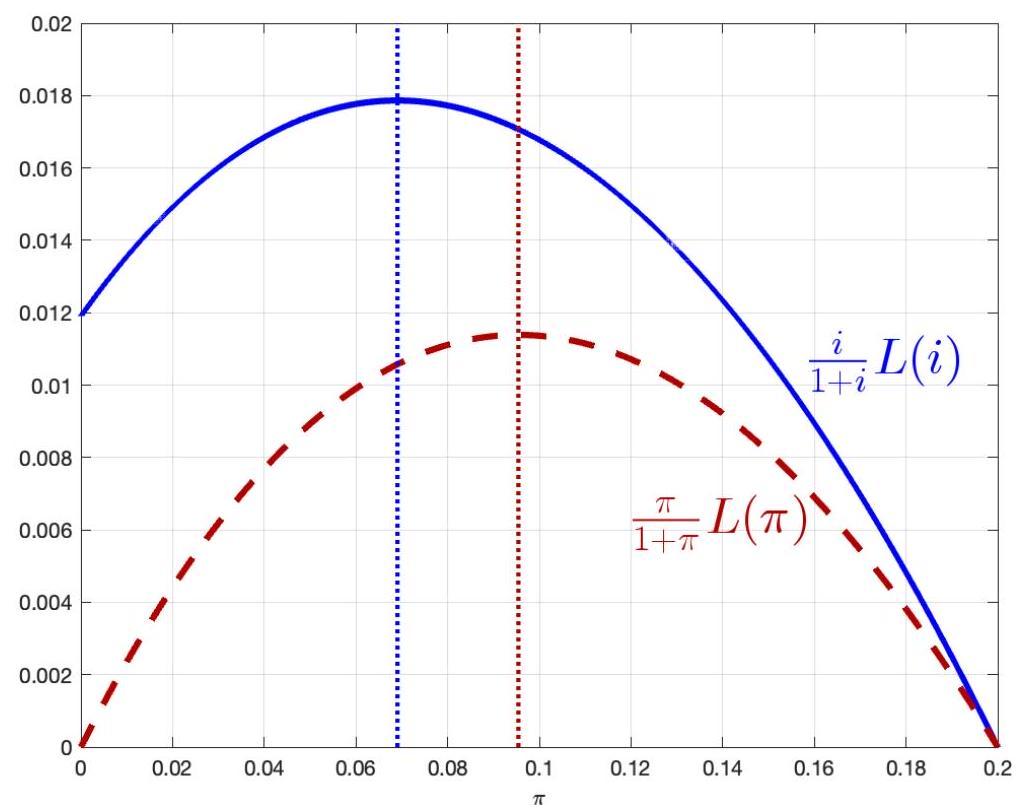
\includegraphics[max width=\textwidth, center]{2024_12_20_6e24ae1385cdc0ea3304g-08}

Figure 1\\
Laffer curves in Sargent-Wallace's "spectacular" example. The bottom dashed curve represents the traditional Laffer curve $\frac{\pi}{1+\pi} L(\pi)$. The top solid curve represents $\frac{i}{1+i} L(i)$ (expressed in terms of $\pi$ using $1+i=(1+\pi)(1+r)$ for fixed $r=0.05$ ).\\
in all periods, so that $i_{t}<\bar{i}_{t}$ for all $t \geq 0$. In that case, it is not possible to increase interest rates marginally, as the left side of (2) is increasing in interest rates. Indeed, for marginal changes we find ourselves in the case of Result \#1, with a tradeoff in inflation across periods. However, one can still engineer increases in interest rates (hence, inflation) by considering discrete changes: for any $t \geq 1$ replace $i_{t, t+1}$ with $i_{t, t+1}^{\prime}>\bar{i}_{t}>i_{t, t+1}$ where $\frac{i_{t, t+1}}{1+i_{t, t+1}} L_{t}\left(i_{t, t+1}\right)=\frac{i_{t, t+1}^{\prime}}{1+i_{t, t+1}^{\prime}} L_{t}\left(i_{t, t+1}\right)$. This amounts to a jump from the good side of the Laffer curve to the bad side of the Laffer curve. ${ }^{11}$

These observations relate to the "spectacular" example in Sargent and Wallace. They showed that inflation could rise in all periods, despite a lower initial money growth rate. We see that there are a number of ways for inflation to rise in all periods, all requiring a decreasing segment in the alternative Laffer curve. Figure 1 shows the traditional Laffer curve (bottom dashed line) and the alternative curve (top solid line) using the money demand in Sargent and Wallace. In their example, some inflation rates lie to the right of the peak of the alternative Laffer curve $\frac{i}{1+i} L(i)$. As discussed below, their example combined marginal changes as well as a discrete jump to the bad side of the Laffer curve.

QR\\
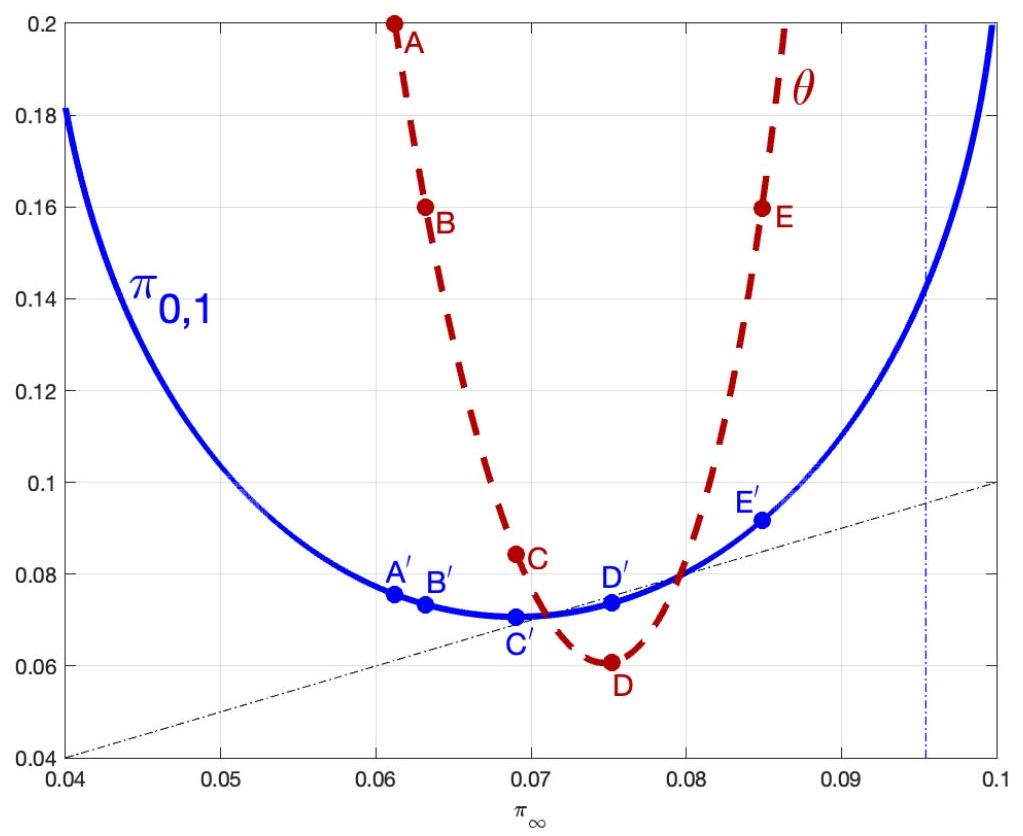
\includegraphics[max width=\textwidth, center]{2024_12_20_6e24ae1385cdc0ea3304g-09}

Figure 2\\
Equilibria for a simple example. The solid curve represents $\pi_{0,1}$ as a function of $\pi_{2,3}=\pi_{3,4}=\cdots=\pi_{\infty}$. The dashed curve shows the implied growth rate of money $\theta=M_{1,2} / M_{0,1}-1$ as a function of $\pi_{\infty}$.

An Illustration. I now illustrate these possibilities and connect them to the spectacular example provided by Sargent and Wallace. I also offer a variant example that reinforces their conclusions.

I explore the set of equilibria for a simple example where money demand is stationary $L_{t}=L$, given by the linear specification from Sargent and Wallace as used in Figure 1. I study equilibria with constant inflation from $t=2$ onwards: $\pi_{t-1, t}=\pi_{\infty}$ for $t=2,3, \ldots \mathrm{I}$ compute $\pi_{0,1}$ as a function of $\pi_{\infty}$ using equation (2) which simplifies to

\begin{equation*}
\left(\frac{i_{0,1}}{1+i_{0,1}}-\frac{1+\omega_{0}}{1+\Delta_{0}}\right) L\left(i_{0,1}\right)+\frac{1}{r} \frac{i_{\infty}}{1+i_{\infty}} L\left(i_{\infty}\right)=D
\end{equation*}

The set of equilibria is depicted as the solid curve in Figure 2, which has a decreasing and increasing portion, respectively associated with the good and bad side of the Laffer curve $\frac{i_{\infty}}{1+i_{\infty}} L\left(i_{\infty}\right)$ in Figure 1. In this example, initial liabilities $\frac{1+\omega_{0}}{1+\Delta_{0}}$ are such that the $t=0$ term $\left(\frac{i_{0,1}}{1+i_{0,1}}-\frac{1+\omega_{0}}{1+\Delta_{0}}\right) L\left(i_{0,1}\right)$ is increasing. Before proceeding, note that the very existence of a minimum for $\pi_{0,1}$ is a simple but powerful manifestation of how fiscal policy constrains what monetary policy can achieve.

Result \#1 applies along the decreasing side of the solid curve. In this region, inflation $\pi_{0,1}$ falls but $\pi_{\infty}$ rises. Result $\# 2$ is associated with the presence of the upward sloping section of this curve. If the original equilibrium lies on the decreasing portion we cannot increase inflation in all periods marginally, but we can do so discretely by considering a jump to the increasing portion of the curve.

To connect my approach with Sargent and Wallace I inspect the initial rate of money growth computed as $1+\theta=M_{1,2} / M_{0,1}=\left(1+\pi_{0,1}\right) L\left(\pi_{\infty}\right) / L\left(\pi_{0,1}\right)$, shown as the dashed curve in the figure. ${ }^{12}$ Moving from point $\mathrm{A}^{\prime}$ to $\mathrm{B}^{\prime}$ is associated with a fall in the growth rate of money $\theta$ from A to B , illustrating Result \#1. A case that illustrates Result \#2 and is akin to Sargent and Wallace's "spectacular" example is represented by a move from point A' to point E', with the growth rate of money falling from A to E. Inflation increases across all periods, despite a lower initial rate of money growth. Note that this requires a discrete jump in the equilibrium selection for a given rate of money growth $\theta$. To see this, decompose the change in two steps: (i) from $\mathrm{A}^{\prime}$ to $\mathrm{B}^{\prime}$ with a fall in $\theta$ (A to B ), and (ii) from $\mathrm{B}^{\prime}$ to $\mathrm{E}^{\prime}$ with no change in $\theta$ ( B to E ). The rise in inflation $\pi_{0,1}$ is then entirely due to the second step from $B$ to $E$, which switches the equilibrium from the decreasing side of the dashed curve to the increasing side. Indeed, if we always select the lowest inflation equilibrium consistent with a given money growth rate $\theta$ (i.e., stay on the decreasing portion of the dashed curve) then we move from A to B , not to E , and we see that inflation $\pi_{0,1}$ falls.

However, the figure shows that it is possible to generate "spectacular" examples without relying on an equilibrium selection switch. For any given growth rate of money there are two equilibria, so let us select the equilibrium with lowest inflation rates. In the figure, this is equivalent to limiting attention to the decreasing side of the dashed curve. Consider a decrease in money growth from C to D : inflation rises in all periods, moving up the solid curve from C' to D'. ${ }^{13}$

Appendix reviews in detail the specific numerical example constructed by Sargent and Wallace as well as a variant, and discusses the connection to the simpler examples discussed here.

\section*{A Seigniorage Perspective}
Sargent and Wallace performed policy variations around an equilibrium, by varying money growth. Previously, I used interest rates as an alternative characterization of monetary policy. Here, I perform local variations in the timing of seigniorage and solve for the equilibrium inflation responses.

\section*{QR}
To do so, start from any equilibrium path $\left\{\bar{s}_{t}, \bar{m}_{t}, \bar{\pi}_{t}\right\}$ satisfying all the equilibrium conditions and take a first-order approximation in the deviations: $\tilde{s}_{t}=s_{t}-\bar{s}_{t}, \tilde{m}_{t}=m_{t}-\bar{m}_{t}$ and $\tilde{\pi}_{t}=\pi_{t}-\bar{\pi}_{t}$. In the main text I simplify expressions by focusing on a stationary initial path $(\bar{s}, \bar{m}, \bar{\pi})$ with stationary money demand. The appendix derives the more general, non-stationary case. The unique bounded solution for inflation is

\begin{equation*}
\tilde{\pi}_{t-1, t}=\frac{1}{\epsilon} \frac{1}{\bar{m}} \sum_{\tau=1}^{\infty} \phi^{\tau} \tilde{s}_{t+\tau}, \quad t=1,2, \ldots \tag{3}
\end{equation*}

with $\tilde{\pi}_{0}$ proportional to $\tilde{\pi}_{1}$, where $\phi \equiv(1+\bar{\pi}) /\left(1+\frac{1}{\epsilon} \frac{1}{1+\bar{\pi}}\right)$ and $\epsilon \equiv-L^{\prime}(\bar{r}+\bar{\pi}) / \bar{m}$ denotes the local semi-elasticity of money demand. For this formula I am assuming $\phi<1$, which is equivalent to being on the increasing portion of the traditional Laffer curve $\frac{\bar{\pi}}{1+\bar{\pi}} L(\bar{\pi})$. Note that $\phi<1$ is ensured for low enough $\epsilon$ or $\bar{\pi}$. When $\phi>1$, equilibria are indeterminate, with a continuum of bounded solutions: even with $\tilde{s}_{t}=0$ for $t=1,2, \ldots$ there are nonzero solutions $\left\{\tilde{\pi}_{t}\right\} .{ }^{14}$ We focus here on the determinate case, $\phi<1$.

Formula (3) embodies a fiscal dominance perspective of inflation, expressing inflation as an increasing function of current and future seigniorage. The relationship is forward looking, not static, because money demand is forward looking. ${ }^{15}$ Only in the limit of inelastic money demand $\epsilon_{t} \rightarrow 0$ does the relationship converge to a myopic one (since $\phi \rightarrow 0$ and $\left.\tilde{\pi}_{t} \rightarrow \tilde{s}_{t} / \bar{m}_{t-1}(1+\bar{\pi})^{2}\right)$.

I now revisit both Sargent-Wallace results, by contrasting the discounted value of seigniorage $\sum_{\tau=1}^{\infty} \phi^{\tau} \tilde{s}_{t+\tau}$ found in formula (3) with $\sum_{t=1}^{\infty}\left(\frac{1}{1+\bar{r}}\right)^{t} \tilde{s}_{t}$ as found in the government budget constraint (1). This comparison depends on $\phi$ versus $\frac{1}{1+\bar{r}}$.

Result \#1 Again. Suppose first that

\begin{equation*}
\phi<\frac{1}{1+\bar{r}}
\end{equation*}

which is guaranteed for low enough $\epsilon, \bar{\pi}$, or $\bar{r}$. Under this condition, if inflation is lowered in some period, then it must be raised in some other periods. We cannot lower inflation across the board: there is a tradeoff.

To see this, consider lowering seigniorage in earlier periods but raising it in future periods to satisfy $\sum_{t=1}^{\infty}\left(\frac{1}{1+\bar{r}}\right)^{t} \tilde{s}_{t}$. This increases inflation in the future as seigniorage rises. However, it lowers inflation in earlier periods, because with $\phi<\frac{1}{1+\bar{r}}$, formula (3) puts relatively less weight on seigniorage in the future. Doing the opposite, pushing seigniorage toward earlier periods, lowers future inflation but raises current inflation because $\phi<\frac{1}{1+\bar{r}}$.

Thus, there is always a trade-off: it is not possible to move inflation in the same direction in all periods.

The preceding argument focused on the term $\sum_{t=1}^{\infty}\left(\frac{1}{1+\bar{r}}\right)^{t} \tilde{s}_{t}$ but set aside the term $\frac{\Delta_{0}-\omega_{0}}{1+\Delta_{0}} L_{0}\left(i_{0,1}\right)$ in the budget constraint (1). However, this does not affect the general logic or conclusions.

Result \#2 Again. Suppose next that

\begin{equation*}
\phi>\frac{1}{1+\bar{r}} .
\end{equation*}

Just as before, a reduction in seigniorage at earlier dates must lead to higher inflation later on because seigniorage must rise at some point in the future. However, because $\phi>\frac{1}{1+\bar{r}}$, the tilting of seigniorage toward the future now leads to an increase in inflation in all periods, since formula (3) puts relatively more weight on seigniorage in the future, which has risen.

While this sounds like a pessimistic message, one can flip things around and engineer a drop in inflation at all times by tilting seigniorage toward the present. As discussed in Section "The Interest Rate Perspective", such a policy "arbitrage" is related to being on the bad side of the Laffer curve $\frac{i}{1+i} L(i)$. Indeed, $\phi(1+r)>1$ holds if and only if $\frac{i}{1+i} L(i)$ is locally decreasing.

\section*{Final Thoughts}
Sargent and Wallace (1981) is rightly celebrated for clarifying how fiscal policy can constrain monetary policy. In the following few decades, most countries successfully designed central bank institutions with independent mandates that have seemingly avoided fiscal dominance, for now. However, vigilant efforts are required to keep these fiscal-monetary constraints at bay, as countries like Argentina serve to remind us.

\section*{Notes}
\begin{enumerate}
  \item Sargent-Wallace impose that after some date $T$ real debt per capita is stabilized at a constant, which implies the no-Ponzi condition, since they assume population grows at a lower rate than the interest.
  \item Taking $M_{0,1}$ as given rules out simple policies that increase $M_{0,1}$ and creates a "jump" in the price level $P_{0}$ that devalues the value of outstanding money and debt. Such a policy has a strong element of surprise since initial money $M_{-1,0}$ and the interest rate $i_{0}$ are taken as given, regardless of the induced jump in the price level $P_{0}$. The policies we consider make money supply predictable
\end{enumerate}

\section*{FEDERAL RESERVE BANK OF MINNEAPOLIS \\
 QR}
one period in advance, although they do not remove all elements of surprise, since $P_{0}$ may still be affected by our policy experiments. However, we can also make similar points on a subset of policy experiments that ensure that $P_{0}$ is unaffected by the policy shifts.\\
3. It is worth clarifying that Sargent-Wallace initially describe their model using real debt, rather than nominal debt. However, they subsequently transform their initial conditions to restrict to nominal debt: see their equation (7) and the discussion surrounding it. In their words and notation, they take the "nominal par value of debt" $\tilde{B}(0)$ (equal to $\left(1+i_{-1,0}\right) B_{-1,0}$ in my notation) as given when performing comparative static exercises throughout the main text. Furthermore, only the initial conditions on debt matters given the arbitrage condition (with perfect foresight) on nominal and real interest rates for all other periods. Thus, in practice, Sargent-Wallace work with nominal debt, as I do here.\\
4. The $1+i_{t, t+1}$ in the denominator adjusts for the fact that the tax is collected a period later.\\
5. The term $1+\Delta_{0}$ in the denominator proportionally affects the initial price level, diluting the real value of initial nominal debt and money balances. In addition, the term $\Delta_{0}$ in the numerator of (1) captures the direct effect of seigniorage in period $t=0$.\\
6. They may even be strictly increasing and unbounded. Being unbounded is difficult to verify, but being strictly increasing or having a peak is a hotly disputed empirical issue.\\
7. A sequence of nominal interest rates then implies a unique sequence for all other variables. Compute inflation using $P_{t+1} / P_{t}=\frac{1+i_{t, t+1}}{1+r_{t, t+1}}$ for all $t=0,1, \ldots$; then compute $P_{0}=M_{0,1} / L\left(i_{0,1}\right)$ since $M_{0,1}$ is exogenously given; finally, compute money $M_{t, t+1}=P_{t} L\left(i_{t, t+1}\right)$ for $t=0,1, \ldots$

Conversely, for any sequence of money that converges to a constant growth rate, there is a unique sequence of prices satisfying the refinement that inflation converges to the long run growth rate in money. Sargent and Wallace impose such a refinement. This then gives a unique sequence of interest rates.\\
8. The initial price level is given by $P_{0}=M_{0,1} / L_{0}\left(i_{0,1}\right)$ and recall that $M_{0,1}$ is given, so inflation is increasing in $i_{0,1}$.\\
9. Note if as is natural $\frac{1+\omega}{1+\Delta}>0$ the term $-\frac{1+\omega}{1+\Delta} L_{0}\left(i_{0,1}\right)$ is increasing and only reinforces this conclusion.\\
10. Since $M_{0,1}$ is given, inflation $\pi_{0}$ at $t=0$ moves in lockstep with $L\left(i_{0}\right)$ and thus with inflation $\pi_{1}$ in period $t=1$.\\
11. I have focused on $t \geq 1$, but after increasing interest rates to $i_{t, t+1}^{\prime}$ for some $t \geq 1$ we can then increase $i_{0,1}$ marginally and decrease $i_{t, t+1}^{\prime}$ marginally to maintain (2). Therefore, it is possible to strictly increase interest rates in all periods $t \geq 0$. In addition, we may also be able to increase $i_{0,1}$ discretely if $\left(\frac{i_{0,1}}{1+i_{0,1}}-\frac{1+\omega_{0}}{1+\Delta_{0}}\right) L_{0}\left(i_{0,1}\right)$ is non-monotone so that there exists $i_{0,1}^{\prime}>i_{0,1}$ with $\left(\frac{i_{0,1}}{1+i_{0,1}}-\frac{1+\omega_{0}}{1+\Delta_{0}}\right) L_{0}\left(i_{0,1}\right)=\left(\frac{i_{0,1}^{\prime}}{1+i_{0,1}^{\prime}}-\frac{1+\omega_{0}}{1+\Delta_{0}}\right) L_{0}\left(i_{0,1}^{\prime}\right)$.\\
12. Recall that $M_{-1,0}$ is given. The growth rate $M_{t, t+1} / M_{t-1, t}$ for $t \geq 2$ equals $1+\bar{\pi}_{\infty}$.\\
13. Indeed, the dashed curve is always decreasing as long as the solid curve is decreasing. This follows from the fact that $\theta=\left(1+\pi_{0,1}\right) L\left(\pi_{\infty}\right) / L\left(\pi_{0,1}\right)$. By implication, the minimum of the dashed curve must be to the right of the minimum for the solid curve. This implies that there is a range of\\
$\pi_{\infty}$ rates with the desired property that inflation rates $\pi_{0,1}$ and $\pi_{\infty}$ rise but the growth rate of money $\theta$ falls.\\
14. Indeed, this is to be expected. When seigniorage is constant is well known that the good side of the Laffer curve is unstable and the bad side is stable, with a continuum of equilibria approaching the bad side of the traditional Laffer curve.\\
15. For example, suppose initially that money supply is constant, with zero seigniorage at all times. Next, consider announcing a doubling of money supply in some future period $t$, with positive seigniorage resulting at this date. This leads to a doubling of the price level at $t$, but inflation cannot be confined to this period. For if it were, money demand would fall in earlier periods, spurring an increase in prices.

\section*{References}
Bassetto, Marco, and Thomas J. Sargent. August 2020. "Shotgun Wedding: Fiscal and Monetary Policy." Annual Review of Economics 12 (1): 659-690.\\
Sargent, Thomas J., and Neil Wallace. 1981. "Some unpleasant monetarist arithmetic." Quarterly Review 5 (Fall).

\section*{Appendix A: Derivation of Present Value Conditions (1) and (2)}
This appendix gives a step by step derivation of the two present value conditions (1) and (2). The starting point for both is the present value condition

\begin{equation*}
\sum_{t=0}^{\infty} q_{t} s_{t}-\frac{\left(1+i_{-1,0}\right) B_{-1,0}}{P_{0}}=D . \tag{4}
\end{equation*}

To get to (1) we note that

\begin{equation*}
\frac{\left(1+i_{-1,0}\right) B_{-1,0}}{P_{0}}=\frac{\left(1+i_{-1,0}\right) B_{-1,0}}{M_{-1,0} \frac{M_{0,1}}{M_{-1,0}}} \frac{M_{0,1}}{P_{0}}=\frac{\omega_{0}}{1+\Delta_{0}} L_{0}\left(i_{0,1}\right)
\end{equation*}

and

\begin{equation*}
s_{0}=\frac{M_{0,1}-M_{-1,0}}{P_{0}}=\frac{M_{0,1}-M_{-1,0}}{M_{-1,0} \frac{M_{0,1}}{M_{-1,0}}} \frac{M_{0,1}}{P_{0}}=\frac{\Delta_{0}}{1+\Delta_{0}} L_{0}\left(i_{0,1}\right) .
\end{equation*}

Thus, we arrive at (1):

\begin{equation*}
\sum_{t=0}^{\infty} q_{t} s_{t}-\frac{\left(1+i_{-1,0}\right) B_{-1,0}}{P_{0}}=\sum_{t=1}^{\infty} q_{t} s_{t}-\frac{1-\omega_{0}}{1+\Delta_{0}} L_{0}\left(i_{0,1}\right)=D .
\end{equation*}

\section*{QR}
To get to (2) start again with (4) and substitute $s_{t}=\frac{M_{t, t+1}-M_{t-1, t}}{P_{t}}$ to get

\begin{equation*}
\sum_{t=0}^{\infty} q_{t}\left(\frac{M_{t, t+1}}{P_{t}}-\frac{M_{t-1, t}}{P_{t}}\right)-\frac{\left(1+i_{-1,0}\right) B_{-1,0}}{P_{0}}=D
\end{equation*}

Collecting the terms $M_{t, t+1}$ in the sum, gives

\begin{equation*}
\sum_{t=0}^{\infty} q_{t}\left(\frac{M_{t, t+1}}{P_{t}}-\frac{q_{t+1}}{q_{t}} \frac{M_{t, t+1}}{P_{t+1}}\right)-\frac{M_{-1,0}}{P_{0}}-\frac{\left(1+i_{-1,0}\right) B_{-1,0}}{P_{0}}=D
\end{equation*}

Next, note that

\begin{equation*}
\sum_{t=0}^{\infty} q_{t}\left(\frac{M_{t, t+1}}{P_{t}}-\frac{q_{t+1}}{q_{t}} \frac{M_{t, t+1}}{P_{t+1}}\right)=\sum_{t=0}^{\infty} q_{t}\left(1-\frac{q_{t+1}}{q_{t}} \frac{P_{t}}{P_{t+1}}\right) \frac{M_{t, t+1}}{P_{t}}=\sum_{t=0}^{\infty} q_{t} \frac{q_{t+1}}{q_{t}} \frac{i_{t, t+1}}{1+i_{t, t+1}} \frac{M_{t, t+1}}{P_{t}}
\end{equation*}

Finally note that

\begin{equation*}
\frac{M_{-1,0}}{P_{0}}+\frac{\left(1+i_{-1,0}\right) B_{-1,0}}{P_{0}}=\frac{M_{-1,0}+\left(1+i_{-1,0}\right) B_{-1,0}}{M_{-1,0} \frac{M_{1,0}}{M_{-1,0}}} \frac{M_{0,1}}{P_{0}}=\frac{1+\omega_{0}}{1+\Delta_{0}} L_{0}\left(i_{0,1}\right)
\end{equation*}

Putting these expressions together gives condition (2),

\begin{equation*}
\sum_{t=0}^{\infty} q_{t}\left(\frac{M_{t, t+1}}{P_{t}}-\frac{q_{t+1}}{q_{t}} \frac{M_{t, t+1}}{P_{t+1}}\right)-\frac{1+\omega_{0}}{1+\Delta_{0}} L_{0}\left(i_{0,1}\right)=D
\end{equation*}

\section*{Appendix B: Spectacular Examples}
This appendix studies the spectacular examples in Sargent-Wallace: where inflation rises in all periods despite an initially lower money growth rate. I discuss a problem of interpretation with the specific parametric example highlighted by Sargent-Wallace, but show there are other similar ones that are free of this problem.

Sargent-Wallace proceeded by parameterizing the initial path for money supply by assuming it grows at some constant rate $\theta$ between period $t=0$ and $t=T$, so that

\begin{equation*}
\frac{M_{1,2}}{M_{0,1}}=\frac{M_{2,3}}{M_{1,2}}=\cdots=\frac{M_{T-1, T}}{M_{T-2, T-1}}=1+\theta
\end{equation*}

Sargent-Wallace focus on equilibria with constant inflation and money growth after $T$, so that $\pi_{t, t+1}=\bar{\pi}$ for $t \geq T-1$. They constrain $\bar{\pi}$ to be to lower than the rate that maximizes

\begin{center}
\begin{tabular}{ccccc}
 & $\theta_{T}$ (bad) & $\theta_{L}$ (good) & $\theta_{T}$ (good) & $\theta_{L}(\mathrm{bad})$ \\
\hline\hline
$t=0$ & $8.4147 \%$ & $8.2503 \%$ & $7.8531 \%$ & $9.6891 \%$ \\
$t=1$ & $8.4129 \%$ & $8.0816 \%$ & $7.7879 \%$ & $9.6783 \%$ \\
$t=2$ & $8.4109 \%$ & $7.8917 \%$ & $7.7150 \%$ & $9.6665 \%$ \\
$t=3$ & $8.4087 \%$ & $7.6771 \%$ & $7.6333 \%$ & $9.6535 \%$ \\
$t=4$ & $8.4063 \%$ & $7.4337 \%$ & $7.5417 \%$ & $9.6394 \%$ \\
$t=5$ & $8.4036 \%$ & $7.1565 \%$ & $7.4386 \%$ & $9.6238 \%$ \\
$t=6$ & $8.4006 \%$ & $6.8392 \%$ & $7.3225 \%$ & $9.6068 \%$ \\
$t=7$ & $8.3973 \%$ & $6.4739 \%$ & $7.1915 \%$ & $9.5881 \%$ \\
$t=8$ & $8.3937 \%$ & $6.0509 \%$ & $7.0434 \%$ & $9.5675 \%$ \\
$t \geq 9$ & $8.3897 \%$ & $5.5573 \%$ & $6.8754 \%$ & $9.5450 \%$ \\
\end{tabular}
\end{center}

Table 1\\
Spectacular equilibria for Sargent-Wallace parameters.\\
the Laffer curve $\frac{\pi}{1+\pi} L_{t}(\pi)$, which with their parameters equals $\sqrt{\frac{\gamma_{1}}{\gamma_{2}}}-1=9.545 \%$. Thus, they introduce an equilibrium refinement requiring inflation to lie on the good side of the Laffer curve for $t \geq T$.

One can solve for the equilibrium as follows. Without loss of generality we normalize $M_{0,1}=1$. This gives us the value of the money supply $M_{t-1, t}$ for $t=1,2, \ldots, T$. Given some $\bar{\pi}$ we then have $P_{T-1}=M_{T-1, T} / L_{T-1}(\bar{\pi})$. We then work backwards solving $P_{t}$ given $P_{t+1}$ using

\begin{equation*}
L_{t}\left(\frac{P_{t+1}}{P_{t}}\right)=\frac{M_{t, t+1}}{P_{t}}
\end{equation*}

for $t=T-2, T-3, \ldots, 0$. This gives us $\pi_{t, t+1}$ for all $t=0,1, \ldots$ (for given $\theta$, the inflation rates derived are monotonically increasing in $\bar{\pi}$ ). This is sufficient (using $1+i_{t, t+1}=$ $\left.\left(1+\pi_{t, t+1}\right)(1+r)\right)$ to evaluate the budget constraint (1) as a function of our guess $\bar{\pi}$ (or we can use the equivalent condition (1)). Denoting the resulting condition by $B(\bar{\pi} ; \theta)=0$, we then solve for equilibrium values for $\bar{\pi}$.

Sargent-Wallace work with a linear money demand function

\begin{equation*}
L_{t}(\pi)=(1+n)^{t}\left(\frac{\gamma_{1}}{2}-\frac{\gamma_{2}}{2}(1+\pi)\right),
\end{equation*}

with parameters $\gamma_{1}=3, \gamma_{2}=2.5, n=0.02$. In addition, they set $r=0.05$ and $\frac{1+\omega_{0}}{1+\Delta_{0}}=$ $\frac{200}{165.65}$. Sargent and Wallace compute two equilibria: one for loose monetary policy $\theta_{L}$ and one for right monetary policy $\theta_{T}<\theta_{L}$ given by

\begin{equation*}
\theta_{L}=0.12 \quad \theta_{T}=0.106
\end{equation*}

\begin{center}
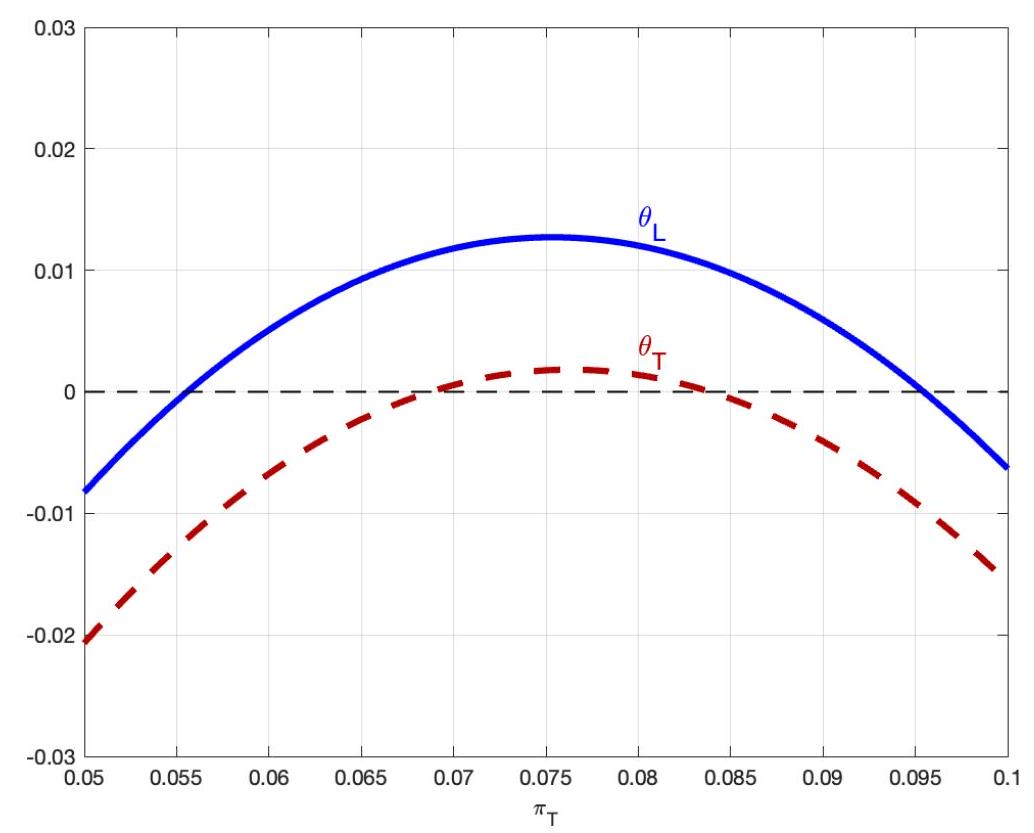
\includegraphics[max width=\textwidth]{2024_12_20_6e24ae1385cdc0ea3304g-17}
\end{center}

Figure 3\\
Equilibrium determination using $G(\bar{\pi}, \theta)=0$. The solid curve uses $\theta_{L}$ and dashed curve uses $\theta_{T}$.

Their two equilibria are shown in the first two columns of Table 1. Comparing these two columns, one sees that inflation is higher in the equilibrium associated with tighter money. Indeed, consistent with the characterization I provided in Section "The Interest Rate Perspective" for the equilibrium with $\theta_{L}$ the inflation rates for $t \leq 5$ lie in the region where the alternative Laffer curve is decreasing (see Figure 1), that is above $6.9047 \%$. This suffices to find equilibria with higher inflation in all periods, as column 1 (generated with $\theta_{T}$ ) illustrates.

Unfortunately, given the parameters of this example, it turns out that there is another equilibrium associated with tight money $\theta_{T}$ that has lower inflation in the first few periods than the equilibrium with loose money $\theta_{L}$. Too see how this is possible, Figure 3 plots the budget constraint condition $G(\bar{\pi}, \theta)$ as a function of $\bar{\pi}$ for the two values of $\theta$. Equilibria are found at the roots, where $G=0$. Because $G$ is quasi-concave there are two such equilibria: one with a low $\bar{\pi}$ and one with a high $\bar{\pi}$. Column 2 corresponds to the low equilibrium of the upper curve. Column 1 corresponds to the high equilibrium of the lower curve.

The inflation rates for the low $\bar{\pi}$ equilibrium with $\theta_{T}$ are shown in the third column (note that $\pi_{9}=\bar{\pi}<9.545 \%$, so the Sargent-Wallace refinement does not rule this equilibrium out). They are lower at all times than in column 1 ; this follows since for given $\theta$, the inflation

\begin{center}
\begin{tabular}{ccccc}
 & $\theta_{T}(\mathrm{bad})$ & $\theta_{T T}(\mathrm{good})$ & $\theta_{T}(\mathrm{good})$ & $\theta_{T T}(\mathrm{bad})$ \\
\hline\hline
$t=0$ & $8.4147 \%$ & $7.8637 \%$ & $7.8531 \%$ & $8.2803 \%$ \\
$t=1$ & $8.4129 \%$ & $7.8108 \%$ & $7.7879 \%$ & $8.2746 \%$ \\
$t=2$ & $8.4109 \%$ & $7.7517 \%$ & $7.7150 \%$ & $8.2682 \%$ \\
$t=3$ & $8.4087 \%$ & $7.6856 \%$ & $7.6333 \%$ & $8.2611 \%$ \\
$t=4$ & $8.4063 \%$ & $7.6116 \%$ & $7.5417 \%$ & $8.2533 \%$ \\
$t=5$ & $8.4036 \%$ & $7.5285 \%$ & $7.4386 \%$ & $8.2446 \%$ \\
$t=6$ & $8.4006 \%$ & $7.4351 \%$ & $7.3225 \%$ & $8.2350 \%$ \\
$t=7$ & $8.3973 \%$ & $7.3301 \%$ & $7.1915 \%$ & $8.2243 \%$ \\
$t=8$ & $8.3937 \%$ & $7.2116 \%$ & $7.0434 \%$ & $8.2125 \%$ \\
$t \geq 9$ & $8.3897 \%$ & $7.0778 \%$ & $6.8754 \%$ & $8.1993 \%$ \\
\end{tabular}
\end{center}

Table 2\\
A variant of the spectacular example in Sargent-Wallace.\\
rates derived by our procedure are monotonically increasing in $\bar{\pi}$. Thus, based on these parameters, one cannot conclude that tighter monetary policy generates higher inflation at all times, since there exists an equilibrium with where inflation is lower for $t \leq 4$. Indeed, if we adopt the common refinement of always choosing the best equilibrium with lowest inflation rates, then tighter monetary policy does not lead to higher inflation in all periods, it lowers inflation initially. This is analogous to the discussion in the text surrounding Figure 2 and the move from $\mathrm{A}^{\prime}$ to $\mathrm{E}^{\prime}$ versus selecting the lowest equilibrium and moving from $\mathrm{A}^{\prime}$ to $\mathrm{B}^{\prime}$.

Fortunately, there are other examples where tighter money leads to higher inflation in all periods, without requiring a shift in the equilibrium selection, for the lowest inflation equilibrium for each $\theta$. I produce an example of this sort as follows. I keep the parameters as before, but now compare $\theta_{T}=0.106$ to "extra-tight" growth $\theta_{T T}=0.105$. The results are presented in Table 2 and Figure 4. Columns 1 and 3 are just as before, but now columns 2 and 4 show the equilibrium for $\theta_{T T}$. Comparing columns 2 and 3 we see that the good equilibrium has higher inflation under extra-tight money $\theta_{T T}$ compared to the equilibrium with $\theta_{T}$. Thus, when comparing these two money growth rates, the tighter policy increase inflation in all periods, even though we have selected the lowest inflation equilibrium for each $\theta$, the lowest intersections in Figure 4. This is analogous to the discussion surrounding Figure 2 and the example variant based on moving in the range between points C and D .

\section*{Appendix C: Linearization and Formula (3)}
This appendix derives a generalized version of formula (3).\\
Seigniorage is given by $s_{t}=m_{t, t+1}-\frac{m_{t-1, t}}{1+\pi_{t}}$ for all $t=0,1, \ldots$ The first order\\
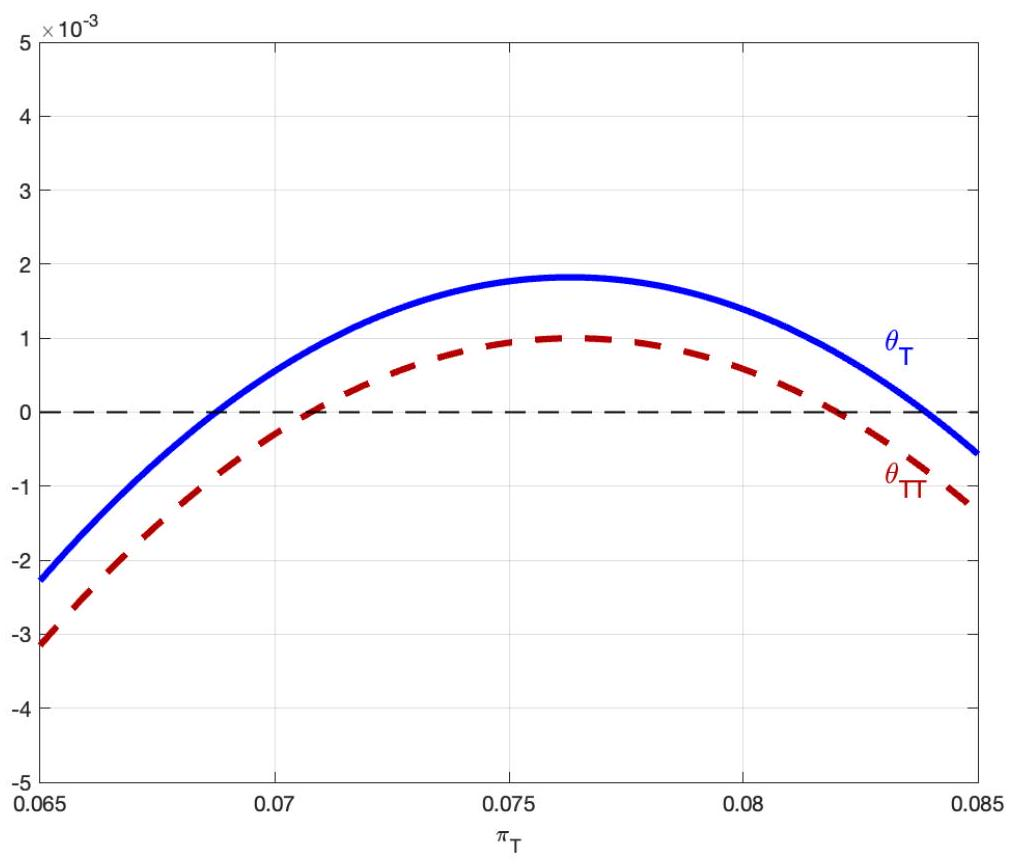
\includegraphics[max width=\textwidth, center]{2024_12_20_6e24ae1385cdc0ea3304g-19}

Figure 4\\
Equilibrium determination using $G(\bar{\pi}, \theta)=0$. The solid curve uses $\theta_{T}$ and dashed curve uses $\theta_{T T}$.\\
approximation gives

\begin{equation*}
\tilde{s}_{t}=\tilde{m}_{t, t+1}-\frac{\tilde{m}_{t-1, t}}{1+\bar{\pi}_{t-1, t}}+\frac{\bar{m}_{t-1, t}}{\left(1+\bar{\pi}_{t-1, t}\right)^{2}} \tilde{\pi}_{t-1, t} \tag{5}
\end{equation*}

For $t \geq 1$, we have $m_{t-1, t}=L_{t-1}\left(\pi_{t-1, t}\right)$ with first-order approximation

\begin{equation*}
\tilde{m}_{t-1, t}=-\epsilon_{t-1} \tilde{\pi}_{t-1, t} \bar{m}_{t-1, t} \tag{6}
\end{equation*}

For $t=0$, nominal money supply is fixed, so real balances are mechanically related to inflation $m_{0,1}=\bar{m}_{0,1} \frac{1+\bar{\pi}_{-1,0}}{1+\pi_{-1,0}}$ with first-order approximation

\begin{equation*}
\tilde{m}_{0,1}=-\bar{m}_{-1,0} \frac{\tilde{\pi}_{-1,0}}{1+\bar{\pi}_{-1,0}} \tag{7}
\end{equation*}

Solving $\tilde{\pi}_{t-1, t}$ in (6) and substituting into (5) gives, for $t \geq 1$,

\begin{equation*}
\tilde{m}_{t-1, t}=\phi_{t}\left(-\tilde{s}_{t}+\tilde{m}_{t, t+1}\right)
\end{equation*}

Recalculating Sargent and Wallace's "Some Unpleasant Monetarist Arithmetic" Werning

\begin{equation*}
\phi_{t} \equiv \frac{1+\bar{\pi}_{t-1, t}}{1+\frac{1}{\epsilon_{t-1}} \frac{1}{\left(1+\bar{\pi}_{t-1, t}\right)}}
\end{equation*}

Assuming $\limsup _{t \rightarrow \infty} \phi_{t}<1$ then

\begin{equation*}
\tilde{m}_{t-1}=-\sum_{s=0}^{\infty} \phi_{t} \phi_{t+1} \cdots \phi_{t+s} \tilde{s}_{t}, \quad t=1,2, \ldots
\end{equation*}

Using (6) once again gives

\begin{equation*}
\tilde{\pi}_{t-1, t}=\frac{1}{\epsilon_{t-1}} \frac{1}{\bar{m}_{t-1}}\left(\sum_{s=0}^{\infty} \phi_{t} \phi_{t+1} \cdots \phi_{t+s} \tilde{s}_{t}\right), \quad t=1,2, \ldots
\end{equation*}

For $t=0$, combining (6) and (7) gives

\begin{equation*}
\epsilon_{0} \tilde{\pi}_{0,1} \bar{m}_{0,1}=\bar{m}_{-1,0} \frac{\tilde{\pi}_{-1,0}}{1+\bar{\pi}_{-1,0}}
\end{equation*}

so that $\tilde{\pi}_{0}$ has the same sign as $\tilde{\pi}_{1}$.


\end{document}